%% ****** Start of file apstemplate.tex ****** %
%%
%%
%%   This file is part of the APS files in the REVTeX 4 distribution.
%%   Version 4.1r of REVTeX, August 2010
%%
%%
%%   Copyright (c) 2001, 2009, 2010 The American Physical Society.
%%
%%   See the REVTeX 4 README file for restrictions and more information.
%%
%
% This is a template for producing manuscripts for use with REVTEX 4.0
% Copy this file to another name and then work on that file.
% That way, you always have this original template file to use.
%
% Group addresses by affiliation; use superscriptaddress for long
% author lists, or if there are many overlapping affiliations.
% For Phys. Rev. appearance, change preprint to twocolumn.
% Choose pra, prb, prc, prd, pre, prl, prstab, prstper, or rmp for journal
%  Add 'draft' option to mark overfull boxes with black boxes
%  Add 'showpacs' option to make PACS codes appear
%  Add 'showkeys' option to make keywords appear
\documentclass[aps,prl,groupedaddress,twocolumn]{revtex4-1}
%\documentclass[aps,prl,preprint,superscriptaddress]{revtex4-1}
%\documentclass[aps,prl,reprint,groupedaddress]{revtex4-1}

\usepackage{graphicx}
\usepackage{epsfig}
\usepackage{subcaption}

\usepackage{amsmath}
\usepackage{amssymb}

\usepackage{dsfont}
\usepackage{bm}
\usepackage{slashed}
\usepackage{cancel}

%package for highlighting text
\usepackage[dvipsnames]{xcolor}
\usepackage{soul} % use \hl{} to highlight text

\usepackage{feynmp}
\usepackage{tikz}
\usepackage{tikz-feynman}
\tikzfeynmanset{
  fermion1/.style={
    /tikz/postaction={
      /tikz/decoration={
        markings,
        mark=at position 0.5 with {
          \node[
            transform shape,
            xshift=-0.5mm,
            fill,
            dart tail angle=100,
            inner sep=1.8pt,
            draw=none,
            dart
          ] { };
        },
      },
      /tikz/decorate=true,
    },
  }
}

%list of my new commands
\newcommand{\beq}{\begin{equation}}

\newcommand{\eeq}{\end{equation}}

\newcommand{\eq}[1]{\begin{equation}\begin{aligned}#1\end{aligned}\end{equation}}

\newcommand{\eqs}[1]{\begin{equation*}\begin{split}#1\end{split}\end{equation*}}

\newcommand{\pp}[2]{\frac{\partial #1}{\partial #2}}

\newcommand{\pa}{\partial}

\newcommand{\da}{\text{d}}

\newcommand{\pd}[2]{\frac{\text{d}#1}{\text{d}#2}}

\newcommand{\Lra}{\Leftrightarrow}

\newcommand{\lra}{\leftrightarrow}

\newcommand{\la}{\leftarrow}

\newcommand{\ra}{\rightarrow}

\newcommand{\Ra}{\Rightarrow}

\newcommand{\La}{\Leftarrow}

\newcommand{\ve}{\varepsilon}

\newcommand{\ttt}[1]{\texttt{#1}}

\newcommand{\R}{\mathds{R}}

\newcommand{\ricci}{\text{\textsc{R}}}

\newcommand{\vp}{\varphi}

\newcommand{\vs}{\varsigma}

\newcommand{\ordo}{\mathcal{O}}

\newcommand{\ham}{\mathds{H}}

\newcommand{\p}{\mathds{P}}

\newcommand{\vk}{\varkappa}

\newcommand{\MF}{\mathcal{F}}

\newcommand{\MS}{\mathcal{S}}

\newcommand{\ML}{\mathcal{L}}

\newcommand{\MJ}{\mathcal{J}}

\newcommand{\MA}{\mathcal{A}}

\newcommand{\cd}{\cdot}

\newcommand{\dgr}{^\dagger}

\newcommand{\pref}[1]{(\ref{#1})}

\makeatletter
\newcommand{\vast}{\bBigg@{4}}
\newcommand{\Vast}{\bBigg@{5}}
\newcommand{\VVast}{\bBigg@{8}}
\makeatother

% You should use BibTeX and apsrev.bst for references
% Choosing a journal automatically selects the correct APS
% BibTeX style file (bst file), so only uncomment the line
% below if necessary.
%\bibliographystyle{apsrev4-1}

\begin{document}

% Use the \preprint command to place your local institutional report
% number in the upper righthand corner of the title page in preprint mode.
% Multiple \preprint commands are allowed.
% Use the 'preprintnumbers' class option to override journal defaults
% to display numbers if necessary
%\preprint{}

%Title of paper
\title{Temperature Comparisons Between Lund, Uppsala, and Luleå}

% repeat the \author .. \affiliation  etc. as needed
% \email, \thanks, \homepage, \altaffiliation all apply to the current
% author. Explanatory text should go in the []'s, actual e-mail
% address or url should go in the {}'s for \email and \homepage.
% Please use the appropriate macro foreach each type of information

% \affiliation command applies to all authors since the last
% \affiliation command. The \affiliation command should follow the
% other information
% \affiliation can be followed by \email, \homepage, \thanks as well.
\author{Nils Björkbäck}
\email[Nils Björkbäck: ]{enter email}
\author{Emil Boman}
\email[Emil Boman: ]{nat14ebo@student.lu.se}
\author{Henrik Olsson}
\email[Henrik Olsson: ]{enter email}
\author{Pavel Oshchepkov}
\email[Pavel Oshchepkov: ]{paul.oshchepkov@icloud.com}
%\homepage[]{Your web page}
%\thanks{}
%\altaffiliation{}
%\affiliation{}

%Collaboration name if desired (requires use of superscriptaddress
%option in \documentclass). \noaffiliation is required (may also be
%used with the \author command).
%\collaboration can be followed by \email, \homepage, \thanks as well.
%\collaboration{}
%\noaffiliation

\date{\today}

\begin{abstract}

\end{abstract}

\maketitle

\section{\label{intro}Introduction}
Things to add here:
\begin{itemize}\setlength\itemsep{-0.2cm}
    \item Intro to subject
    \item some background
    \item goals
    \item what was done (remember to include info about choice of git setup)
    \item short about results
    \item structure of the report.
\end{itemize}

%%%%%%%%%%%%%%%%%%%%%%%%%%%%%%%%%%%%%%%%%%%%%%%%%%%%%%%%%%%%%%%%%%%%%
\section{Data Cleaning}

The datasets, in the form of csv-files, treated in this project contain meta data that need to be removed from the versions given as input to the data processing functions. In order to accomplish this a simple bash script cleanData.sh was used. It first uses the cut command to separate the first 3 columns in the file, which contain data on the format year;time;temperature. It then uses the tail command to to remove metadata at the top of the file.

%%%%%%%%%%%%%%%%%%%%%%%%%%%%%%%%%%%%%%%%%%%%%%%%%%%%%%%%%%%%%%%%%
\section{Number of Winter Days}
%intro, restate goal, present structure of section

This part of the project aimed at comparing the number of winter days, i.e. the number of days with negative average temperature, per year in Lund, Uppsala, and Luleå, during the time period 1964-2022. To accomplish this the number of winter days were calculated and plotted, together with the corresponding centralized moving average over five-year intervals. In addition the relative number of winter days for Lund and Uppsala, using Luleå as the base line, was also determined. The data processing consisted of both a bash script and c++ functions, and the plotting was done using the ROOT framework. In this section begins with a description of the pre-C++ data processing, followed by the C++ data processing and plotting, after which the results are described and analyzed.  

\subsection{Pre-C++ Data Processing}

The first step of the data treatment, after the cleaning process, is the extraction of days with negative temperature, which is done using the bash script negTempDays.sh . This script also introduces the cut off year 1964. This step reduces the size of the datasets to be treated significantly. Similarly to cleanData.sh, the tail command is utilized to do the line cut off. The grep and sort -u commands are then used to track the days with negative temperatures, which are lastly extracted, again using grep.

\subsection{C++ Data Processing and Plotting}

The data processing using C++ is done using the functions \texttt{winterday\_map} and \texttt{winterday\_hist\_fill} in \texttt{winterdays}. The first of these take a csv-file on the format \texttt{date,time,temperature} and determines the number of winter days for each year by calculating the number of days where the sum of the temperature measurements are negative, which corresponds to days with negative average temperatures. The number of winter days for each year is then given as output inside a \texttt{map$<$int year,int temperature$>$}. The second function, \texttt{winterday\_his\_fill}, is then used to insert the data in these maps into the corresponding histogram, and to calculate the centralized moving average over five-year intervals, which is also stored in a histogram.

The plotting of the number of winter days histograms is treated by \texttt{winterday\_hist\_draw}, which draws histograms and moving averages, provided in two vectors, on a canvas and then saves the canvas as a pdf. For the plotting of relative number of winter day histograms, \texttt{rel\_winterday\_hist\_gen} is used. This function takes two maps containing years with corresponding number of winter days and inserts the quotient of the number of days into a histogram, using the years as bins. The histogram is then drawn on a canvas, which is saved to a pdf.

\subsection{Results}

things to add here:

\begin{itemize}\setlength\itemsep{-0.2cm}
    \item present the number of winter days plot. done
    \item number of days Lunc$<$Uppsala$<$Luleå.
    \item significant spike in 2009.
    \item Previous periods of few winter days in Lund, though shorter periods than what we have now.
    \item Uppsala: two spikes in recent years, but other than that slightly fewer winter days.
    \item moving averages decreasing over time (particluarly noticeable in Luleå and Uppsala data) $\ra$ climate change.
\end{itemize}
The number of winter days per year recorded in Lund, Uppsala, and Luleå, from 1964 to 2022, is shown as histograms in figure \ref{fig:winterdays}. Included in the figure is also the centralized moving average over five-year intervals for each histogram. 
\begin{figure}[h!]
    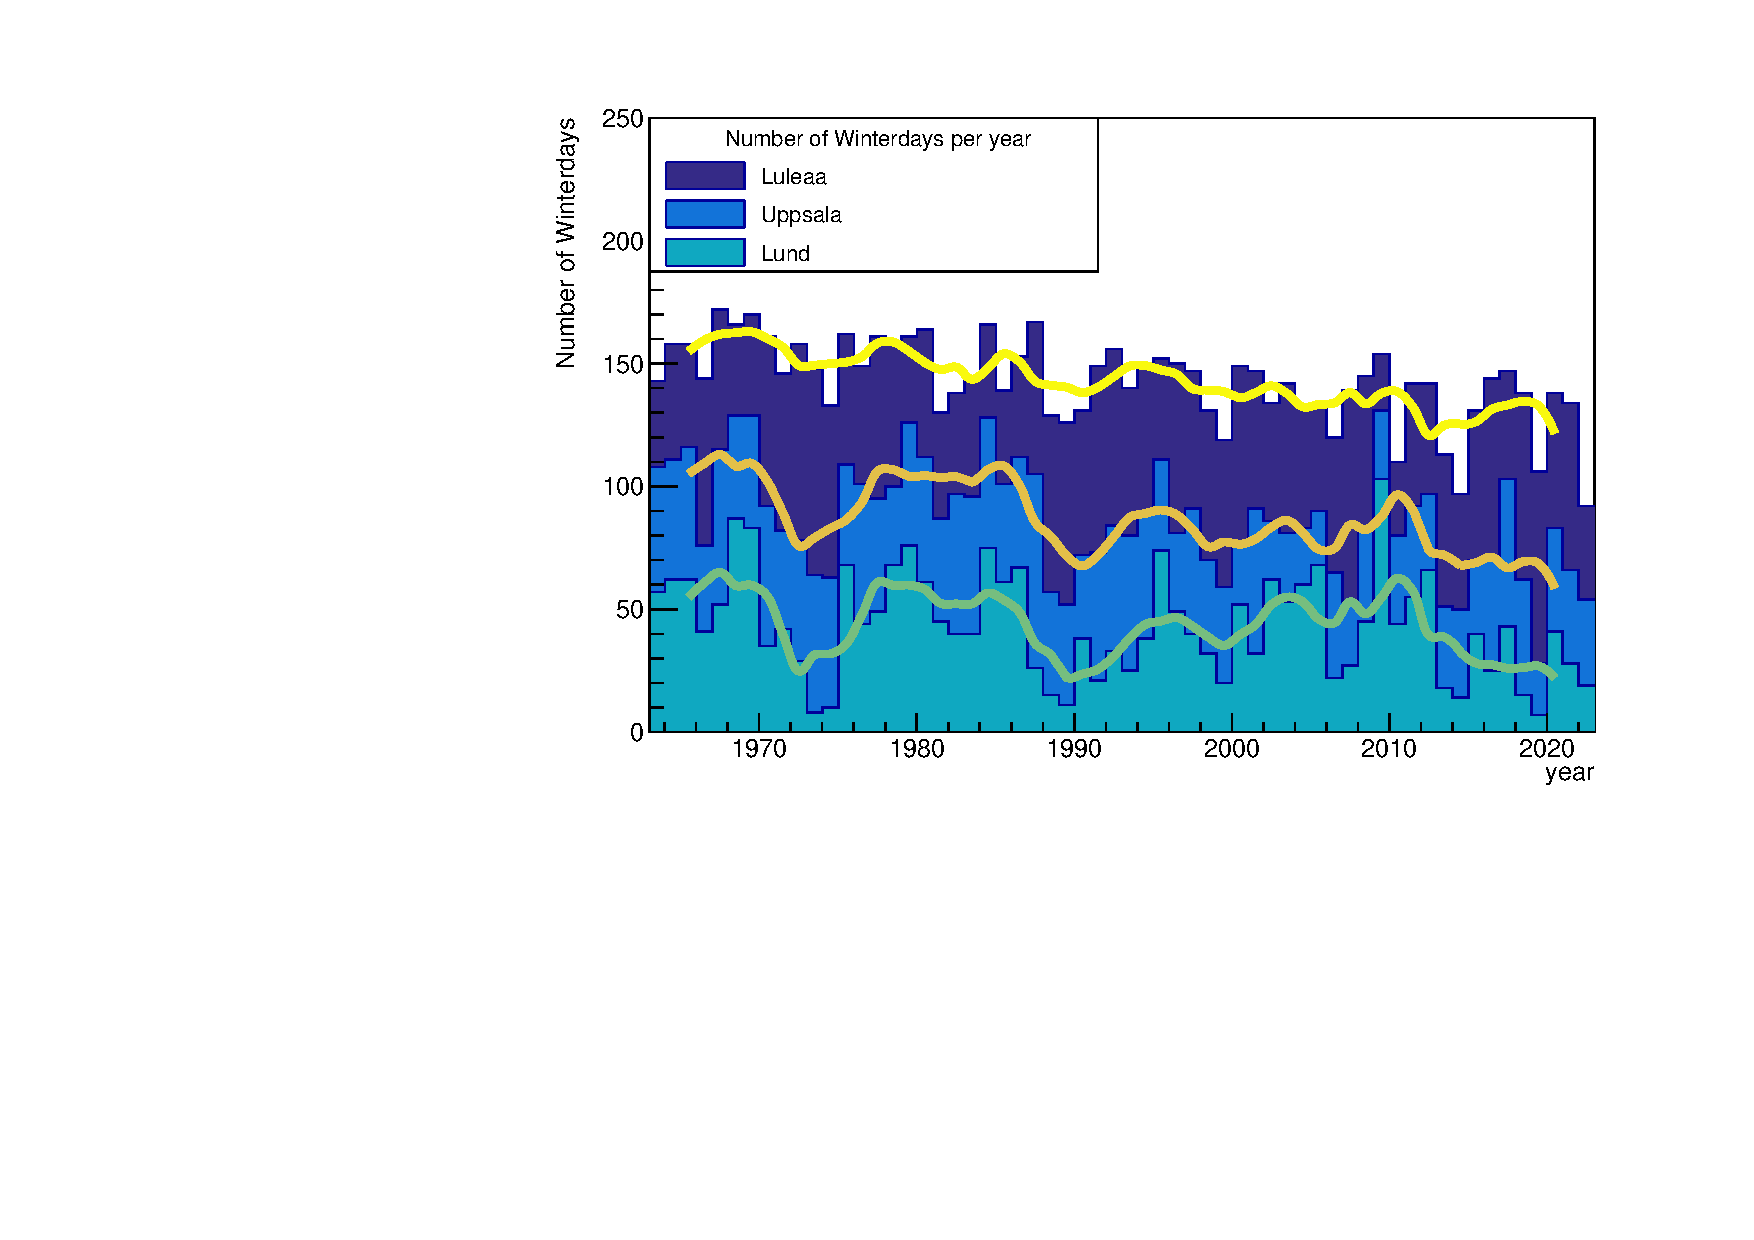
\includegraphics[scale=0.5,trim=0.5cm 0.3cm 0.5cm 1cm,clip]{winterday_hist.pdf}
    \caption{The number of winter days from 1964 to 2022 for Lund, Uppsala, and Luleå. For each histogram the centralized running average over five-year intervals is also shown.}
    \label{fig:winterdays}
\end{figure}

things to add here:

\begin{itemize}\setlength\itemsep{-0.2cm}
    \item Present relative number of winter days plot. done
    \item Spike in 2009 is a relative spike, particularly in Lund data.
    \item Lund has larger relative diff between high and low points than Uppsala.
\end{itemize}
The relative number of winter days between Lund and Luleå, from 1964 to 2022, is shown in figure \ref{fig:rel_lund}, and the counterpart for Uppsala is shown in figure \ref{fig:rel_uppsala}.

\begin{figure}[h!]
    \begin{subfigure}{0.45\textwidth}
            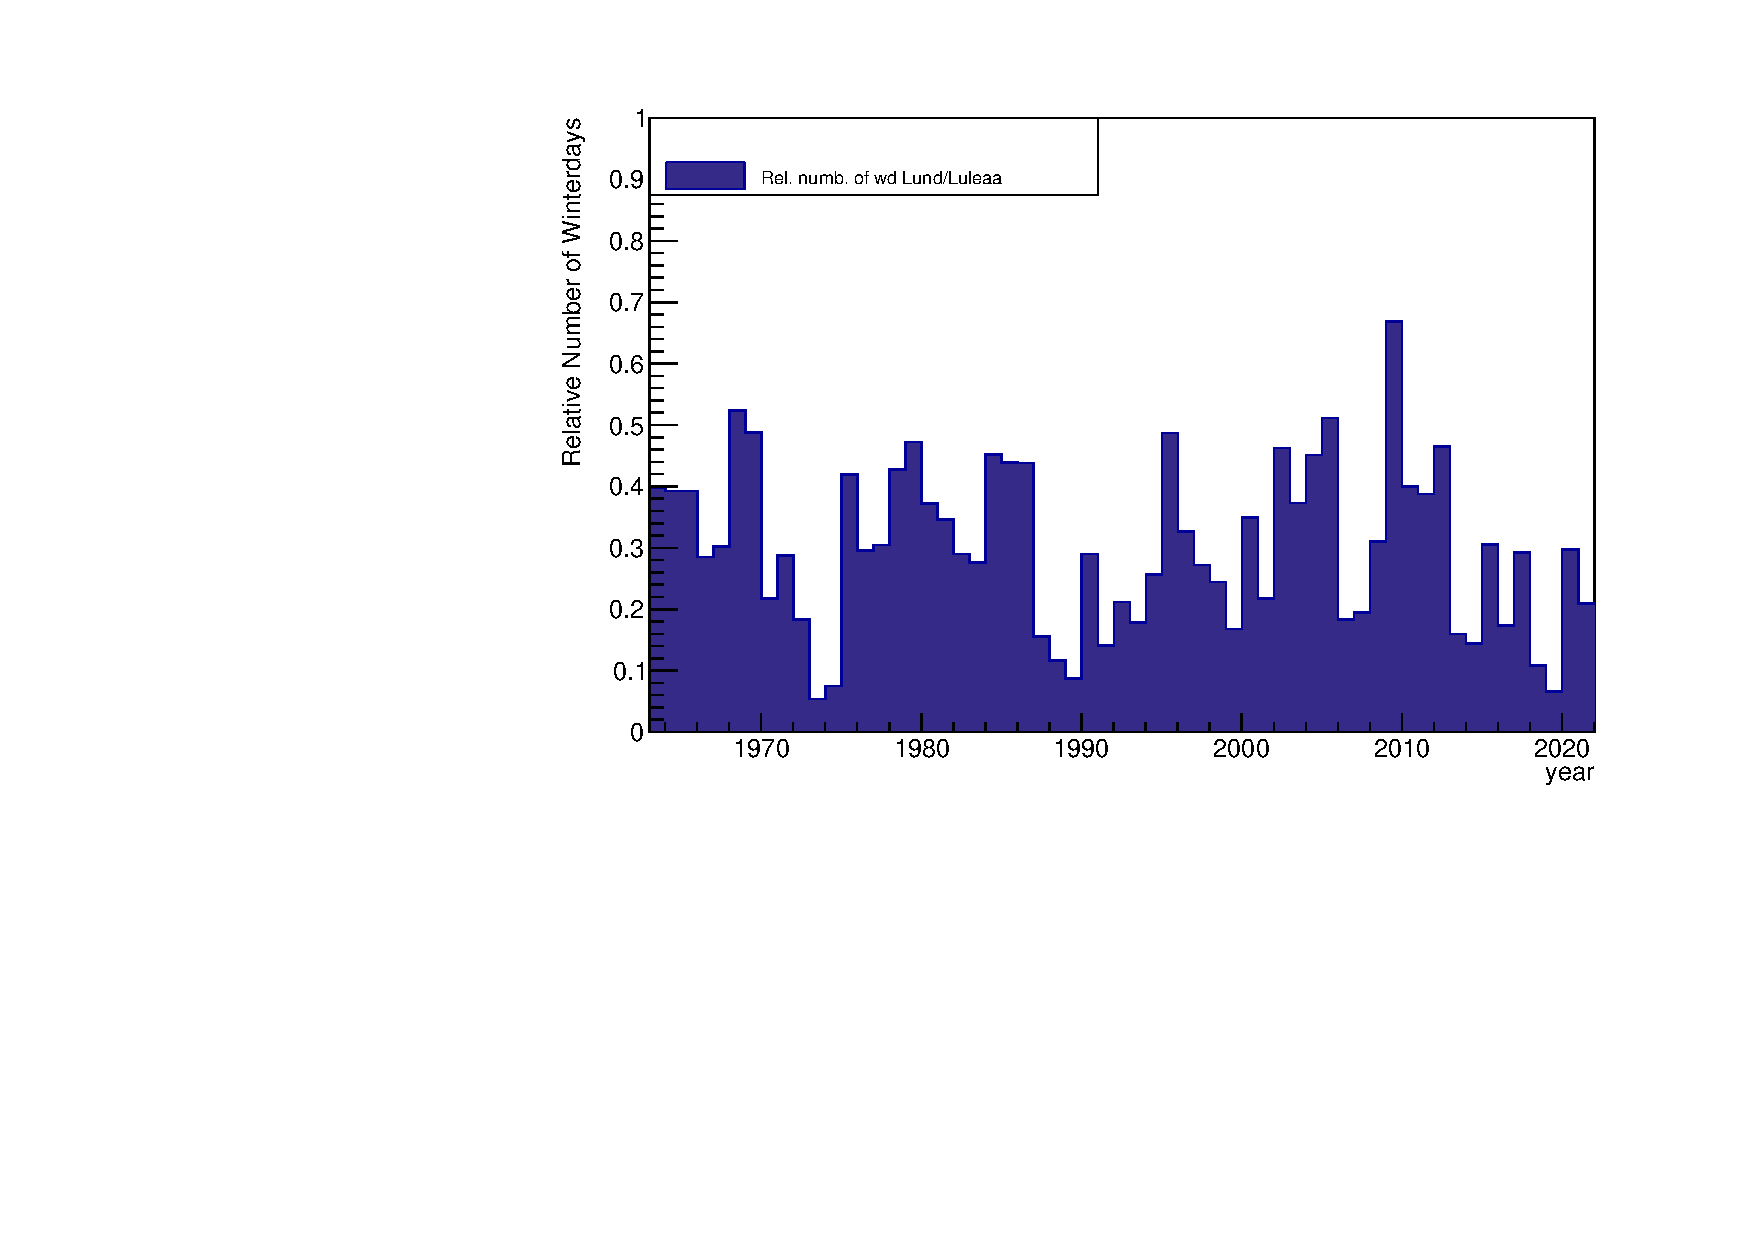
\includegraphics[width=\textwidth]{rel_Lund_hist.pdf}
            \caption{The relative number of winter days between Lund and Luleå from 1964 to 2022.}
            \label{fig:rel_lund}
    \end{subfigure}
    \hfill
    \begin{subfigure}{0.45\textwidth}
            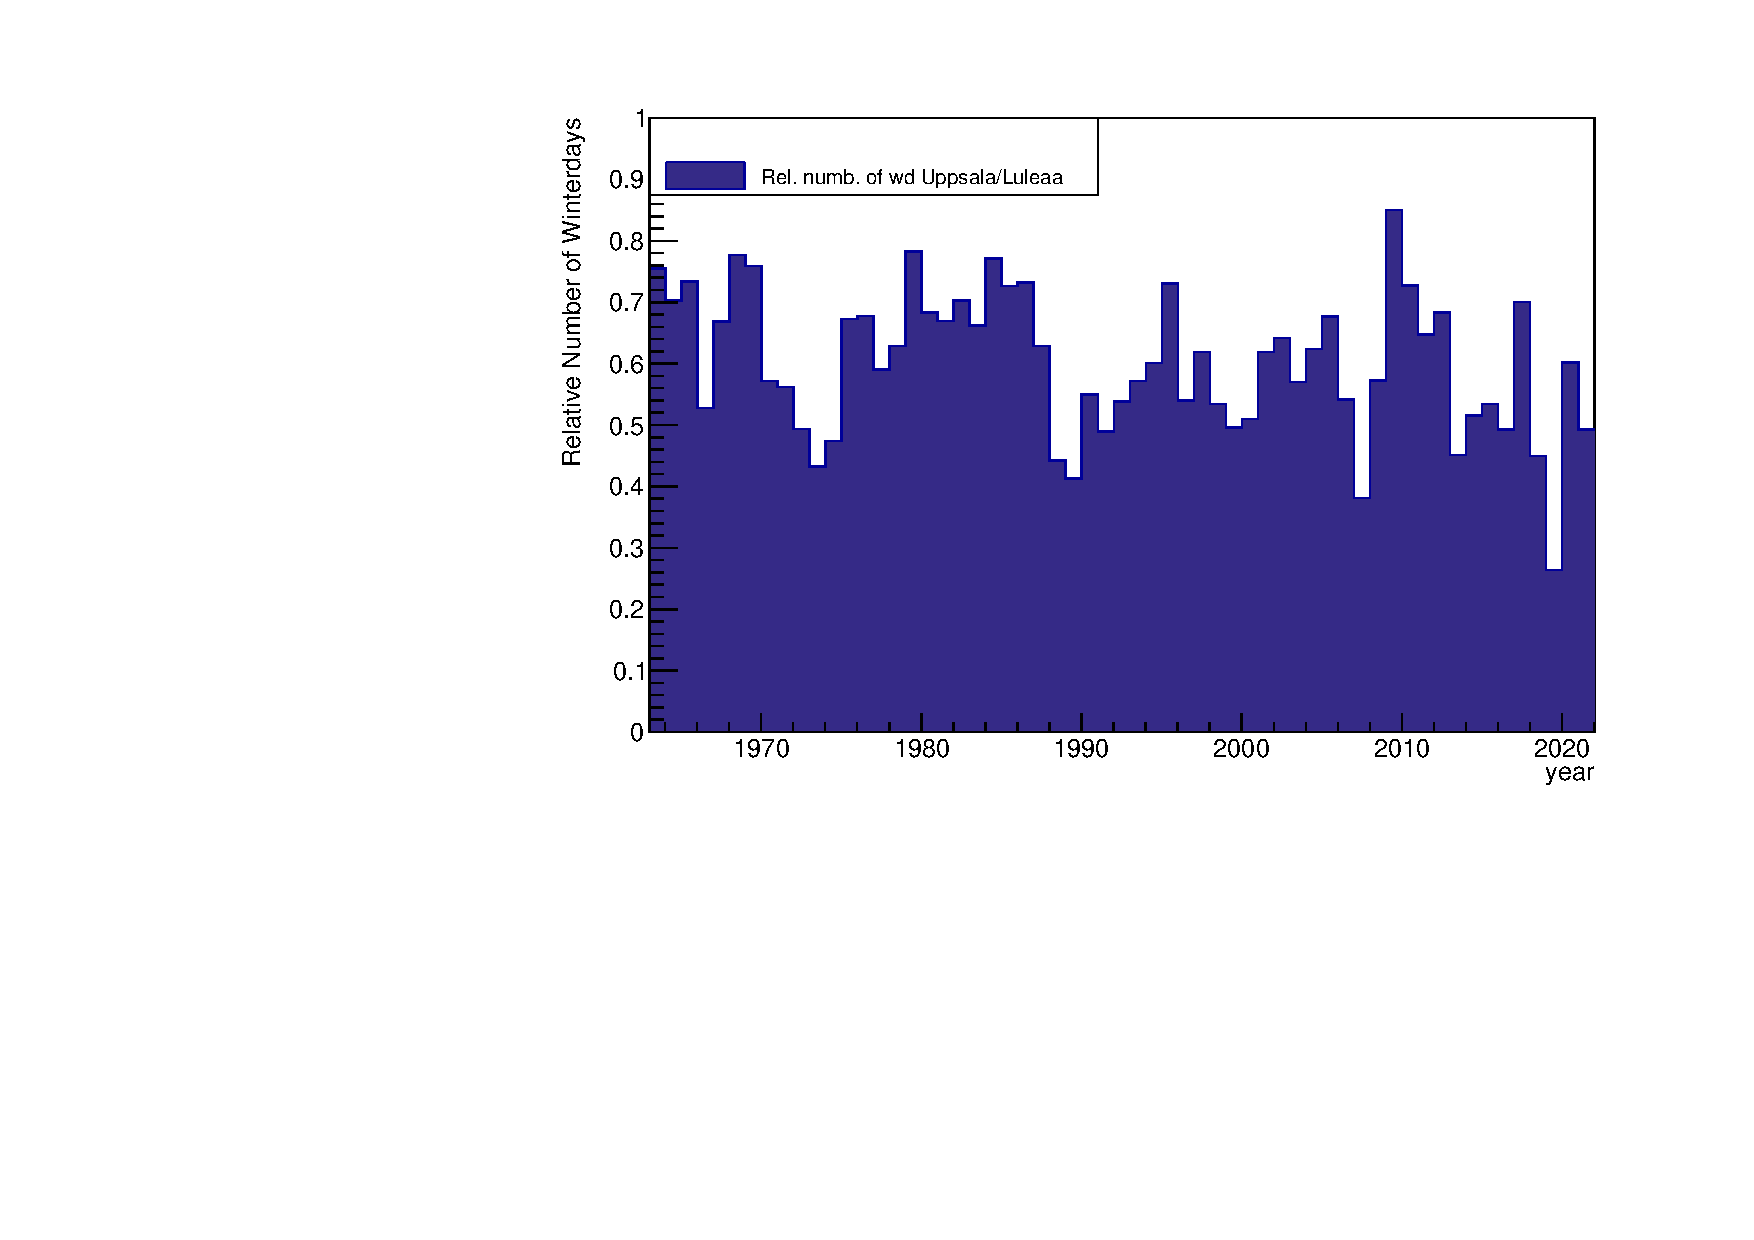
\includegraphics[width=\textwidth]{rel_Uppsala_hist.pdf}
            \caption{The relative number of winter days between Uppsala and Luleå from 1964 to 2022.}
            \label{fig:rel_uppsala}
    \end{subfigure}
    \caption{The relative number of winter days with Luleå as a reference.}
    \label{fig:rel_winterdays}
\end{figure}

\newpage

%%%%%%%%%%%%%%%%%%%%%%%%%%%%%%%%%%%%%%%%%%%%%%%%%%%%%%%%%%%%%%%%%%%
\section{Average monthly temperature difference between Lund and Lulea}
\subsection{Introduction}
The main goal of this sub-project was to look into the monthly temperature difference between Lund and Luelea over a the same time period. Throughout the data analysis plots were prepared for average monthly temperature throughout the common time period for which the data was present which is 1949-01-01 to 2022-12-31. If the temperatures stayed consistent over this years the data can compiled into average temperature difference for every month. 
\subsection{Data Preparation}
The data was first cleaned using the shell script for cleaning the data. The a new script cut\_to\_size.sh was written in order the cut the data to same date range. The script takes in data multiple data sets and ask for a start and end date. Produces a new file with the header from the original file and with the data in between the provided start and end date. Both of the data sets were cut down to common range. 
\subsection{Data Analysis Using C++}
All of the data analysis and plotting using C++ was is done in the tempDelta.cxx script.
During the data analysis the data was first organized into two hash maps of std::string dates and double total temperatures in totalTemperaturePerDay(std::string file) method and another hash map of std::string dates and int measurement amount in the measurnmentsPerDay method. Those hash maps were then used to find the average temperature each day from multiple measurements for each day this was again organized into a hash map and then formatted to use date::year\_month\_day as the key value. That was done in the averageTemperaturePerDay and averageTemperaturePerDayFormatted methods. This was used to calculate the monthly average temperature in the avergeTempearaturePerMonth method. The output hash map was used to prepare the first set of plots for average monthly temperature in Lulea and Lund in the PlotData method. Then the temperature difference was calculated in the GetTemperatureDelta method and plotted in PlotDelta delta. Lastly the data was compiled to find the average temperature difference for each month in GetAverageTotalDeltaByMonth method and plotted in PlotDeltaByMonth.
\subsection{Results}
The first results are just the average monthly temperatures over the years for both cities. Looking at this it can be clearly seen that the average temperature in Lund is pretty consistently above 0 throughout the year while the temperature in Lulea varies significantly from summer to winter.
\begin{figure}[h!]
    \begin{subfigure}{0.45\textwidth}
            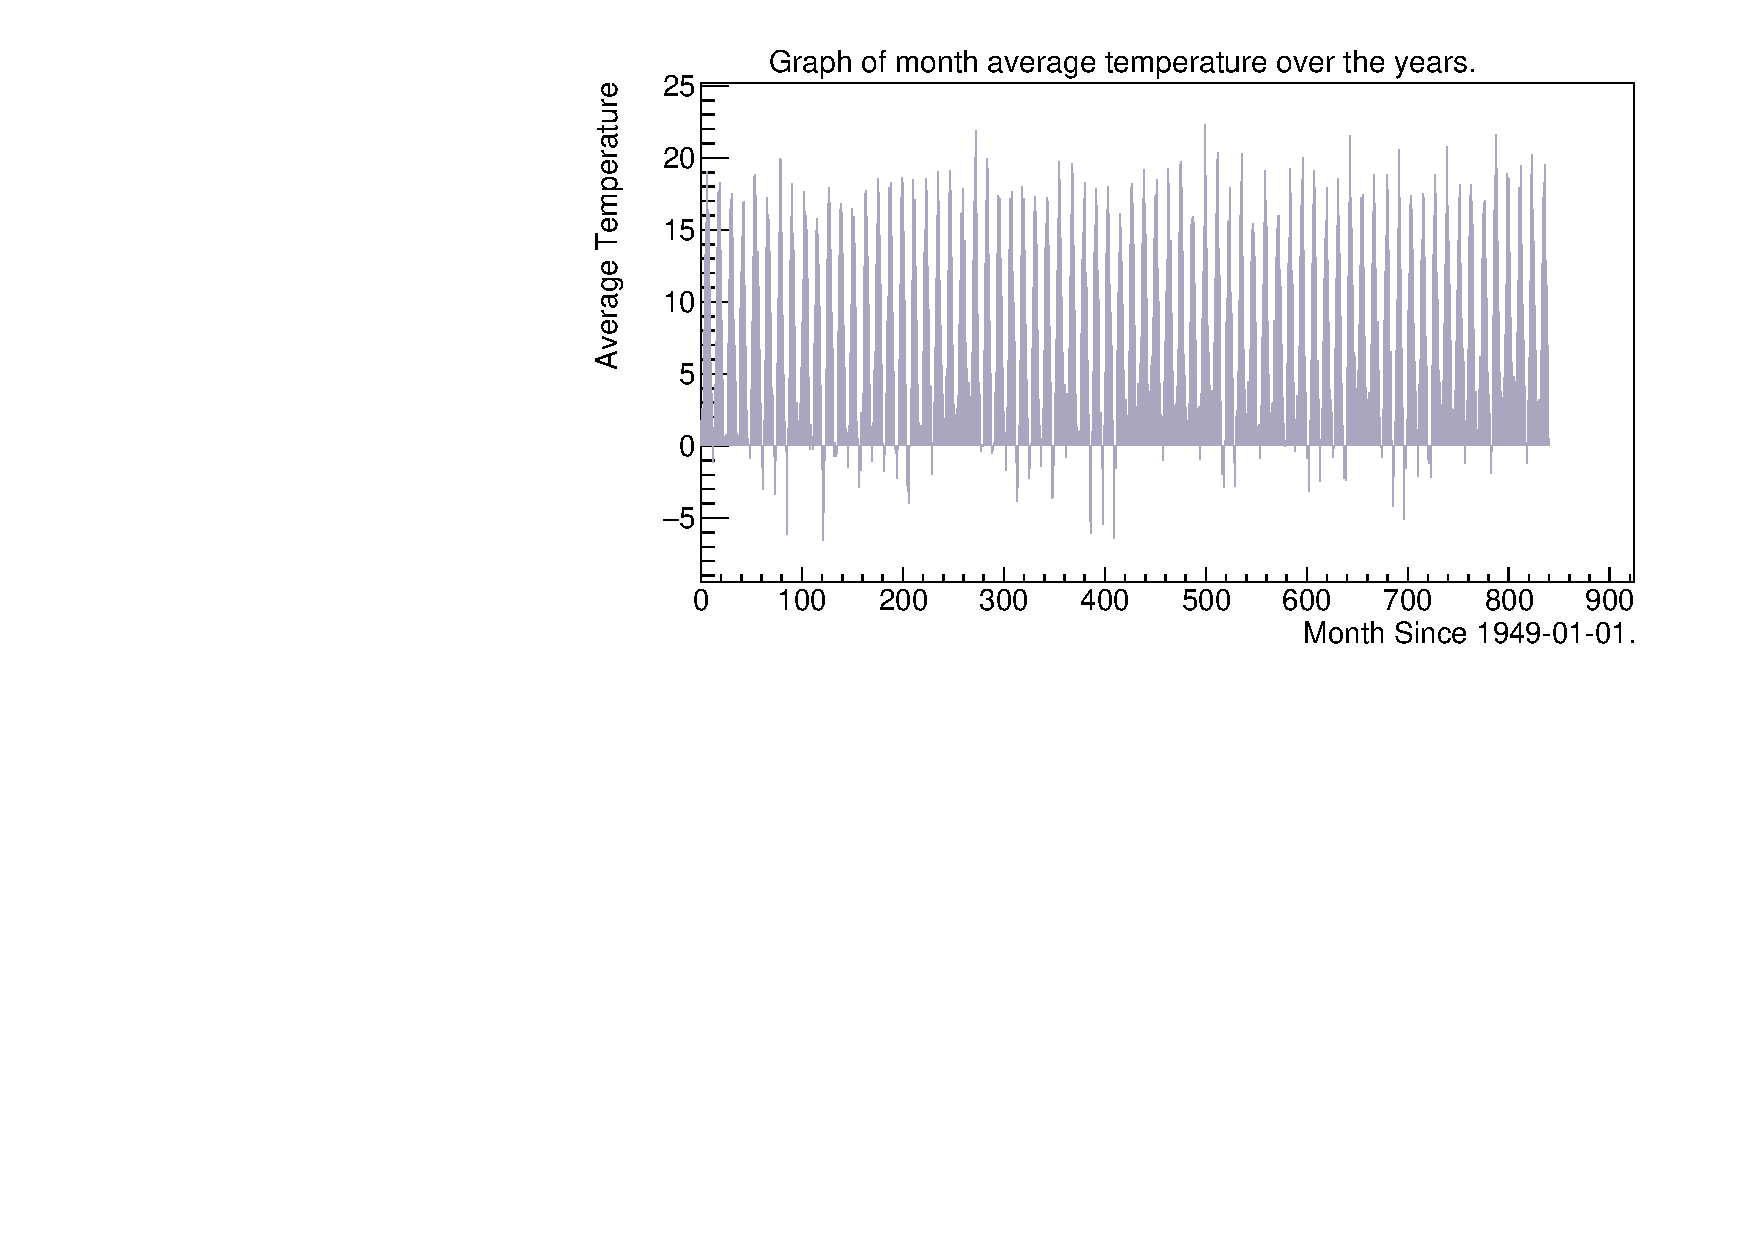
\includegraphics[width=\textwidth]{monthlyAverageTemperatureLund.pdf}
            \caption{Monthly average temperature from 1949-01-01 in Lund.}
            \label{fig:monthlyLund}
    \end{subfigure}
    \hfill
    \begin{subfigure}{0.45\textwidth}
            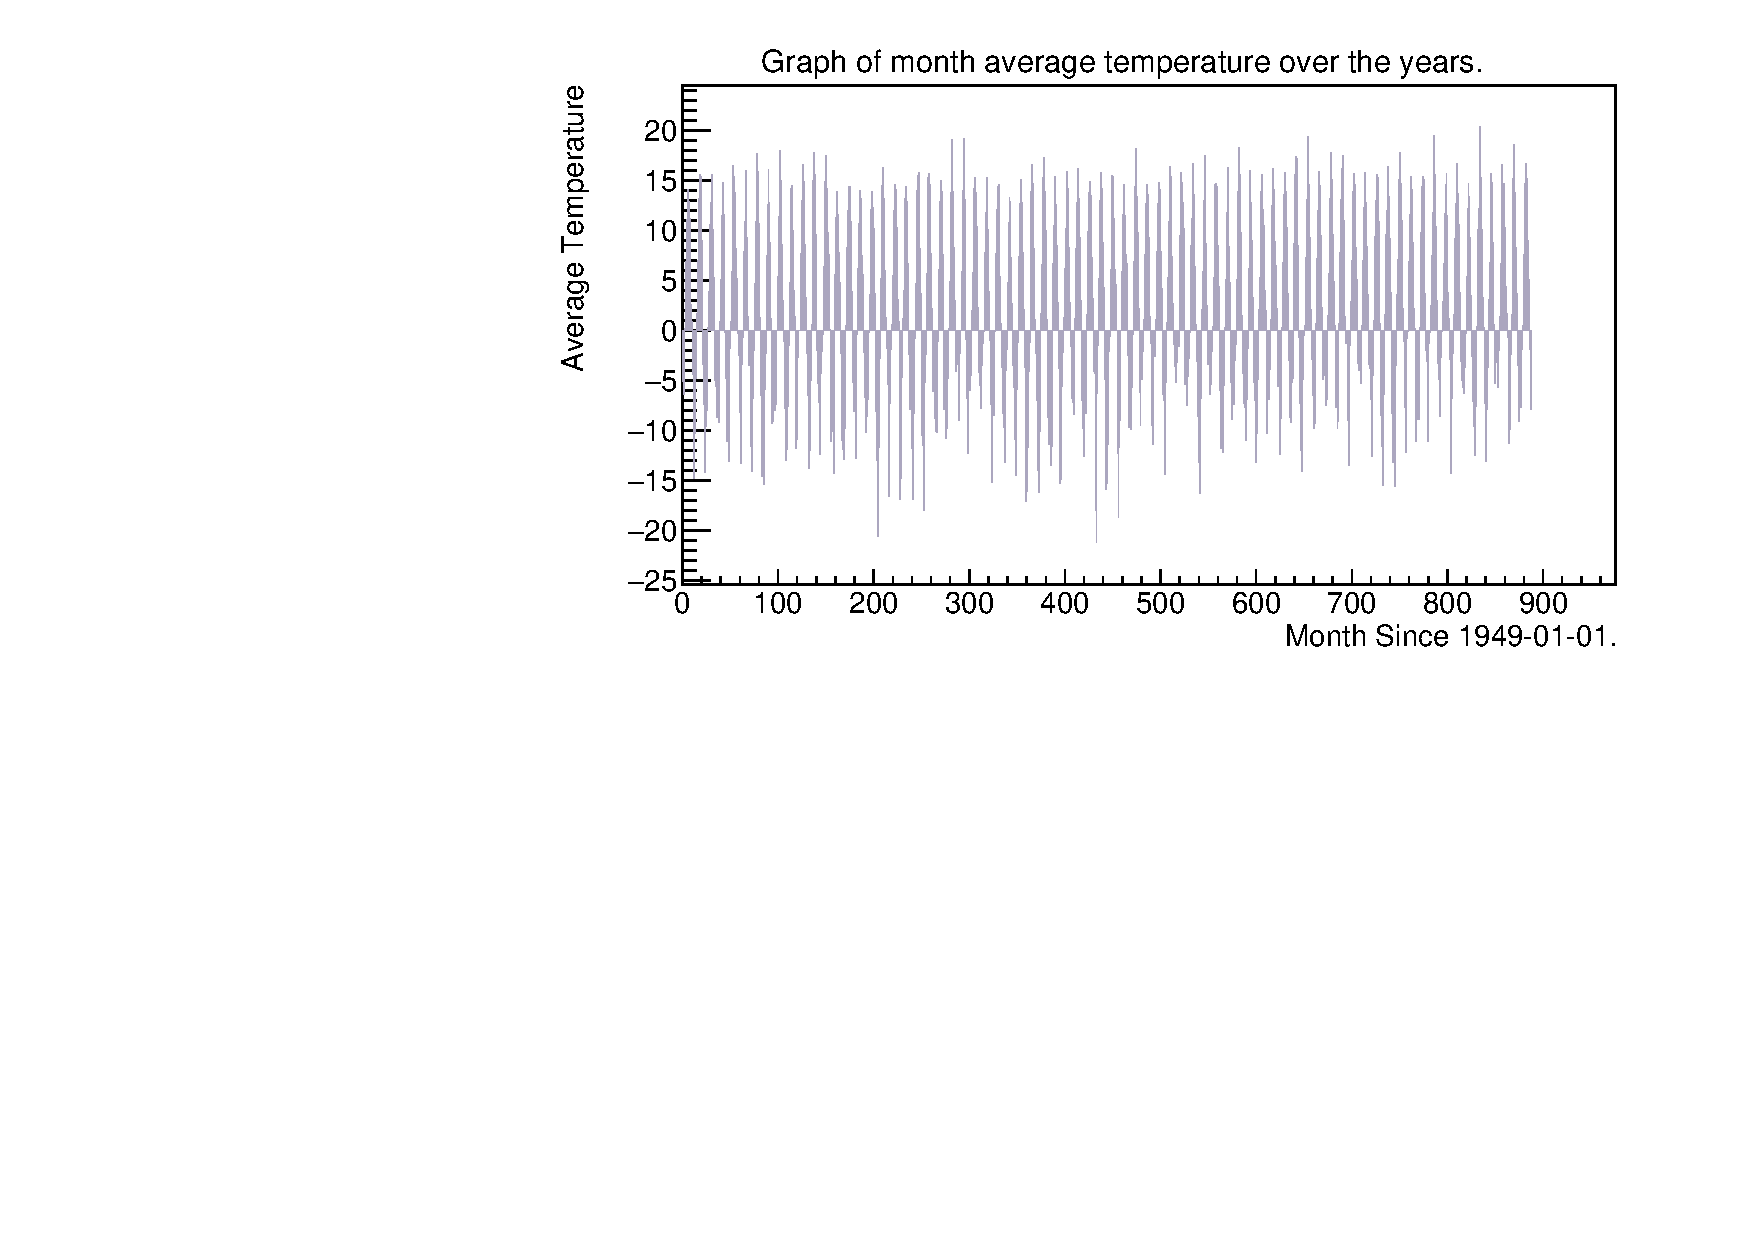
\includegraphics[width=\textwidth]{monthlyAverageTemperatureLulea.pdf}
            \caption{Monthly average temperature from 1949-01-01 in Lulea.}
            \label{fig:monthlyLulea}
    \end{subfigure}
    \caption{Monthly average temperatures in Lund and Lulea.}
    \label{fig:monthlyTemp}
\end{figure}

The second result was from looking at the temperature difference between the two cities as Lund - Lulea.
\begin{figure}[h!]
    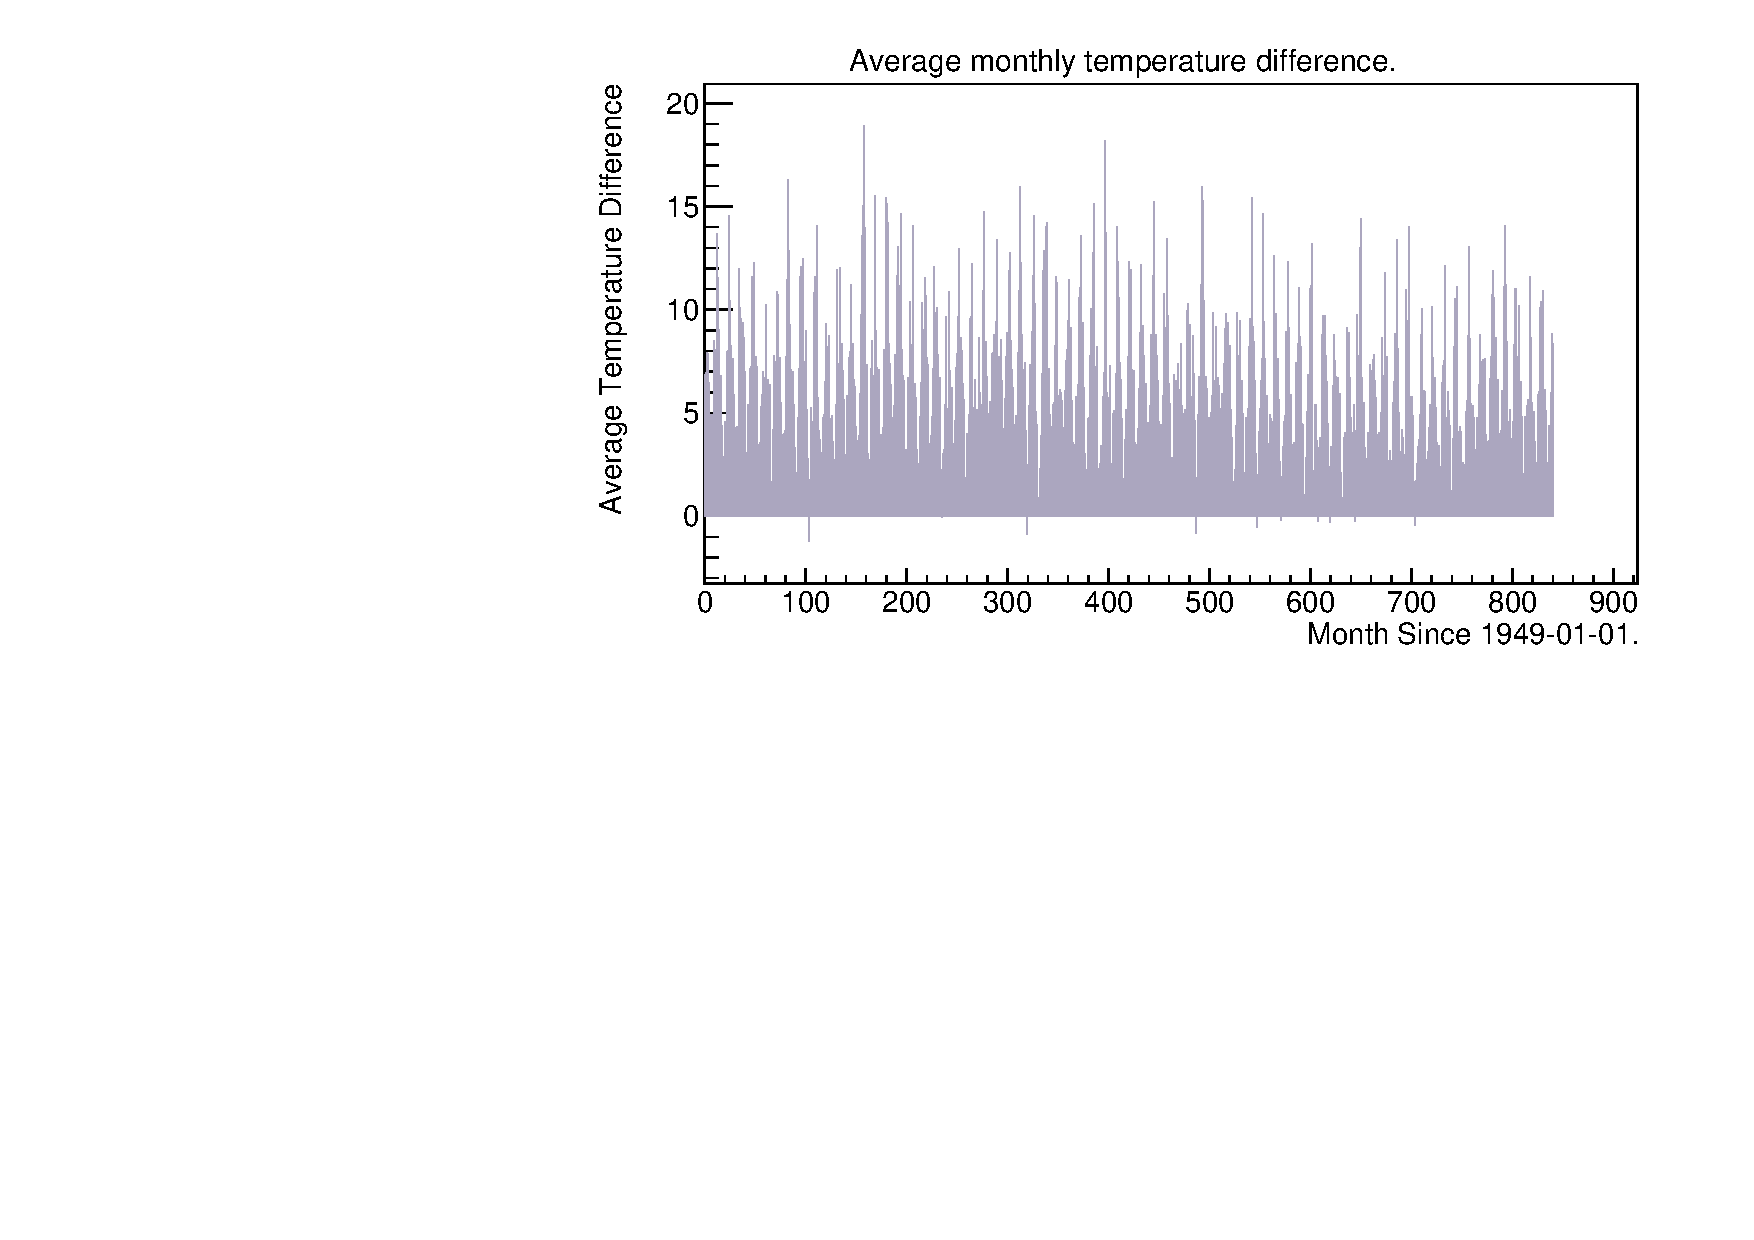
\includegraphics[width=0.45\textwidth]{temperaturedeltaLundLulea.pdf}
    \caption{Temperature delta Lund - Lulea from 1949-01-01.}
    \label{fig:monthlyDelta}
\end{figure}
The final result of the sub-project is the average temperature delta between the cities for each month. This result shows that the temperature difference is greatest in the cold month and goes to its minimum during July. The reason for this is that as already discussed before the temperature in Lund stays relatively consistently positive throughout the year while Lulea changes drastically during the year meaning that the temperature difference is smallest during the warm month of the year.
\begin{figure}[h!]
    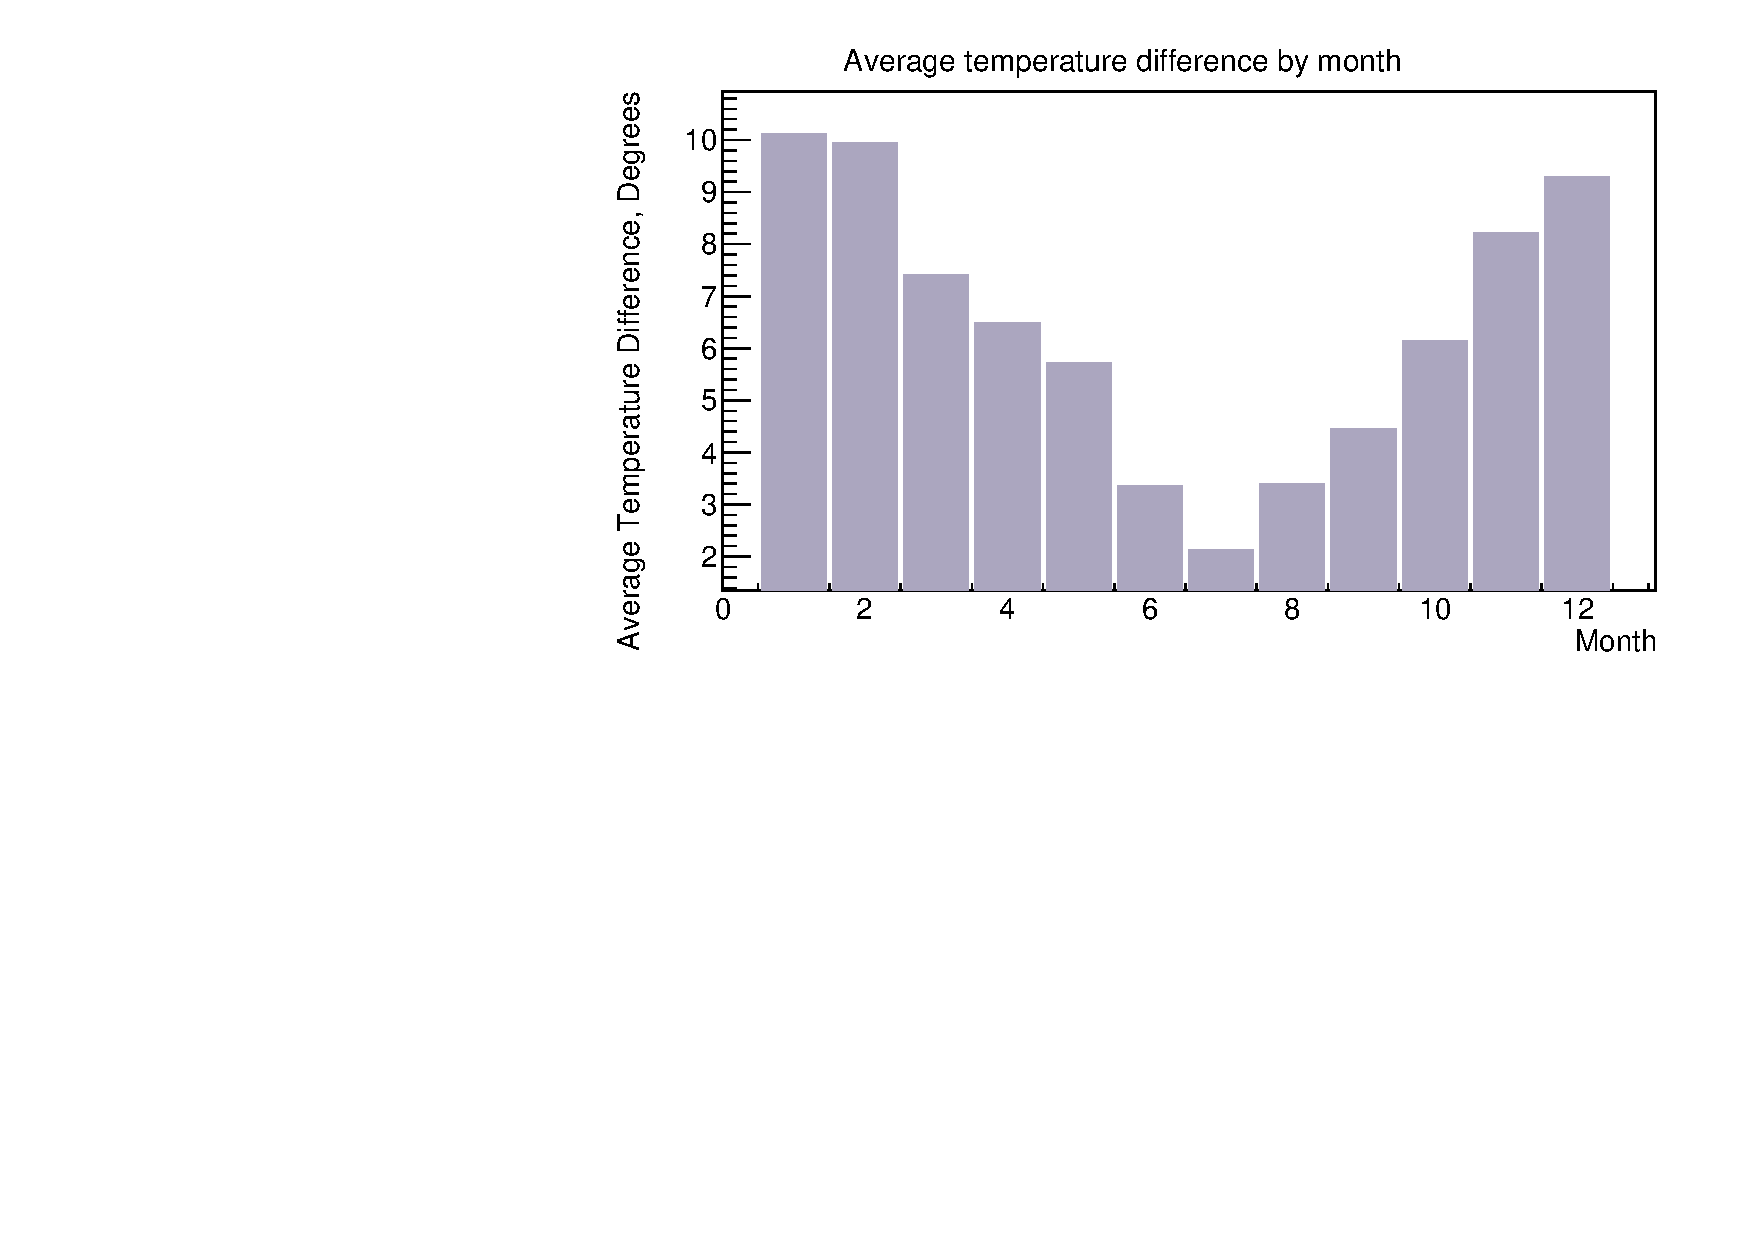
\includegraphics[width=0.45\textwidth]{tempDeltaByMonth.pdf}
    \caption{Monthly Temperature Delta.}
    \label{fig:tempDelta}
\end{figure}




\section{Subproj. 3}

\section{Subproj. 4}



\section{Conclusions}


\section{acknowledgments}


\begin{thebibliography}{99}

\bibitem{smhi}
Sveriges meteorologiska och hydrologiska institut, \textit{Ladda ner meteorologiska observationer}, SMHIs öppna data, URL: https://www.smhi.se/data/meteorologi/ladda-ner-meteorologiska-observationer/\#param=airtemperature-Instant,stations=core .
\end{thebibliography}

\end{document}
%
% ****** End of file apstemplate.tex ******